\documentclass[xcolor=table]{beamer}

\usetheme[secheader,compress]{Madrid} %Primary theme

\usepackage{verbatim}
\usepackage{graphicx}

%% UTM Colors
\definecolor{UTMblue}{rgb}{0.043137, 0.137254, 0.254901}
\definecolor{UTMorange}{rgb}{1.0, 0.509803, 0}

\setbeamercolor{palette primary}{bg=UTMblue,fg=white}
\setbeamercolor{palette secondary}{bg=UTMblue,fg=white}
\setbeamercolor{palette tertiary}{bg=UTMblue,fg=white}
\setbeamercolor{palette quaternary}{bg=UTMblue,fg=white}
\setbeamercolor{structure}{fg=UTMblue} % itemize, enumerate, etc
\setbeamercolor{section in toc}{fg=UTMblue} % TOC sections
\setbeamercolor{title}{fg=UTMorange}

\setbeamercolor{subsection in head/foot}{bg=UTMorange,fg=white}

%%%%%%%%%%% BEGIN MACROS %%%%%%%%%%%%%%%%%%
% frameT: Frame with title
\newcommand{\frameT}[2]{\frame{\frametitle{#1} #2}}

% frameF: Fragile frame with title
\newcommand{\frameF}[2]{
  \begin{frame}[fragile]
    \frametitle{#1}
    #2
  \end{frame}
}

% frameTop: Frame aligned t the top
\newcommand{\frameTop}[2]{\frame[t]{\frametitle{#1} #2}}


\newcommand{\tab}{\hspace{1cm}}

\newcommand{\spaceor}{\hspace{5pt} \textbf{or} \hspace{5pt}}

%%%%%%%%%%% END MACROS %%%%%%%%%%%%%%%%%%%%



\begin{document}

\title{Project Spellda}

\author{Steven Gray, James Nail, and Logan Brown}
\institute{UT-Martin}
\date{\today}

%%%%%%%%%%% BEGIN TITLE %%%%%%%%%%%%%%%%%%
\frame{\titlepage}

 %\section{Outline}
%%%%%%%%%%%% END TITLE  %%%%%%%%%%%%%%%%%%


\section{Introduction}
\frameT{Motivation} {
	\bigskip
  \begin{enumerate}
		\item We all shared an interest in gaming and wanted to make a game
			\bigskip
    \item We wanted to step out of our comfort zone with something we may use in the future.
  \end{enumerate}

  \bigskip
}

\section{Goals}

\frameT{Project Goals} {
	\begin{enumerate}
		\item 3 Levels: Tutorial, Overworld, and Dungeon
		\bigskip
		\item 4-6 different enemies, 2 melee and 2-4 ranged
		\bigskip
		\item 4 different elements to control
		\bigskip
		\item 8 unique effects to modify the spells
	\end{enumerate}
}


\frameT{Stretch Goals}{
	\begin{enumerate}
		\item Secret Boss(/es)
		\bigskip
		\item More dungeons
		\bigskip
		\item Expanded Overworld
		\bigskip
		\item Elemental weaknesses/resistences
		\bigskip
		\item More effects/elements
	\end{enumerate}
}


\frameT{Technologies}{
	\begin{enumerate}
		\item Godot/GDScript
		\item This is the core tech we've been using. Has done everything we need it to and then some.
			\bigskip
			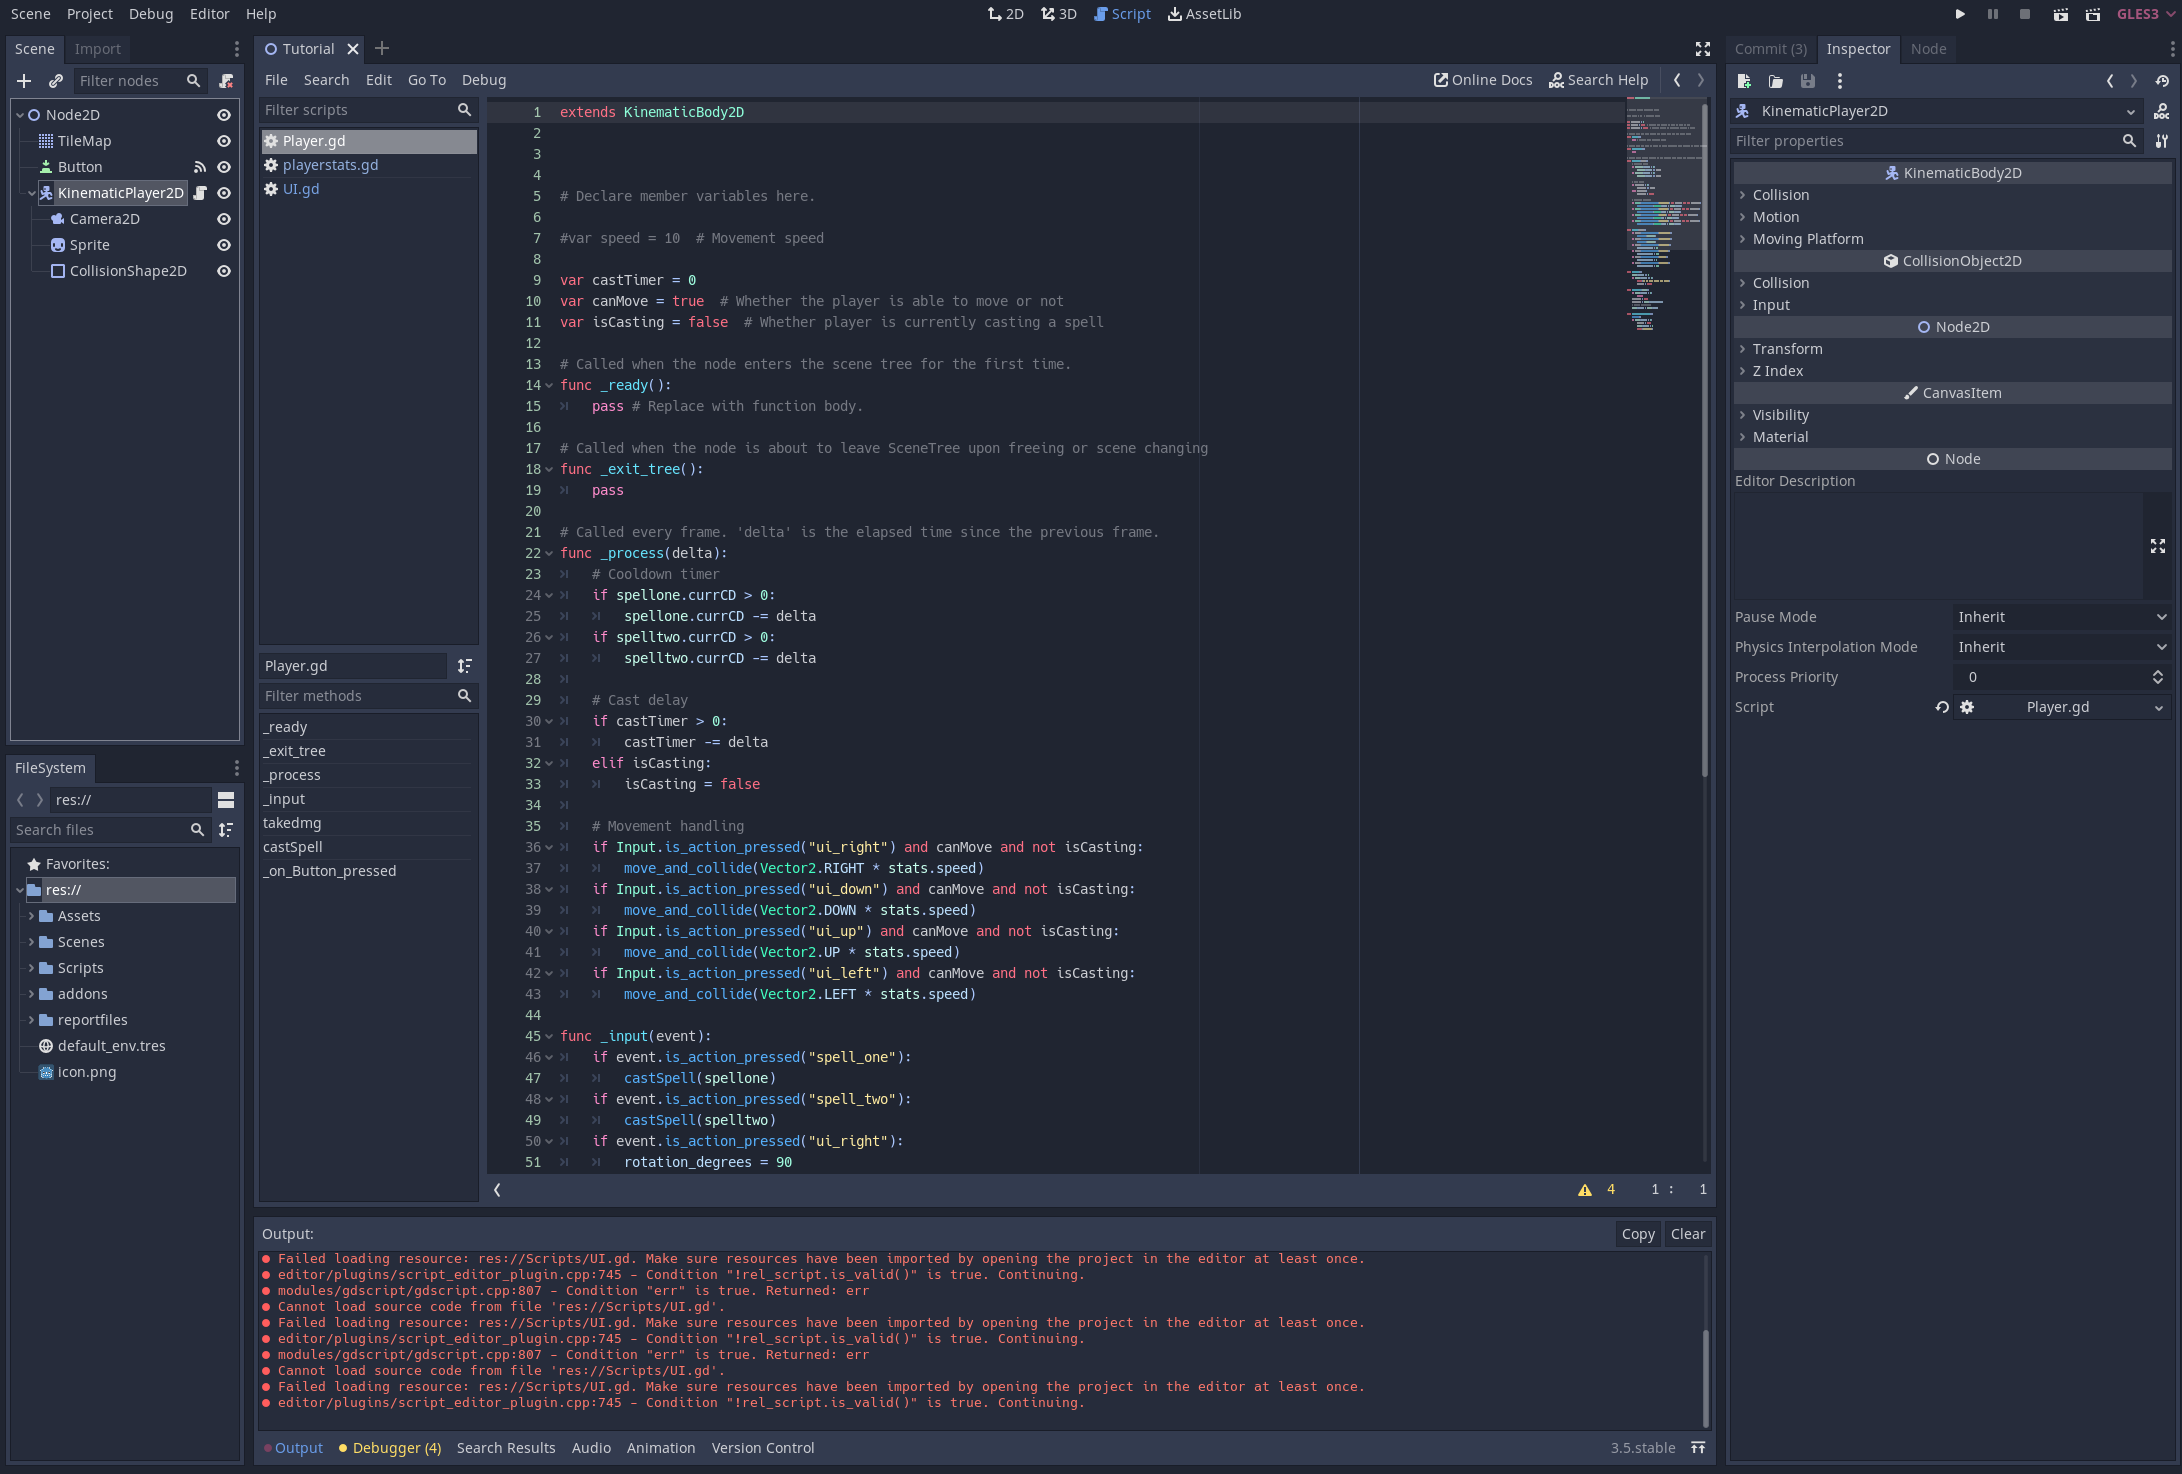
\includegraphics[width=.7\linewidth]{figures/godotscreenshot.png}
	\end{enumerate}
}

%%%%%%%%%%%%%%%%%%%%%%%%%%%%%%%%%%%% Commented-Out code starts here


\begin{comment}
\begin{frame}[fragile]
\frametitle{Family Tree Knowledge Base}
Facts:
\begin{verbatim}
Verbatim is a great way of enumerating code/algorithmic ideas.
\end{verbatim}
\end{frame}


\frameT{How to include images} {
  %% \includegraphics[width=.7\linewidth]{figures/image.pdf}
}


\begin{frame}[fragile]
  \frametitle{Social Network Graph}
  \begin{figure}[ht]
    \begin{minipage}[b]{0.53\linewidth}
      \centering
      Minipages are a great way to
    \end{minipage}
    \hspace{0.5cm}
    \begin{minipage}[b]{0.4\linewidth}
      \centering
      Line up side-by-side content.

    \end{minipage}
  \end{figure}
  
\end{frame}

\end{comment}


%%%%%%%%%%%%%%%%%%%%%%%%%%%%%%%%%%%% Commented-Out code ends here


\frameT{Demo} {
Here is a look into what we have!
\bigskip

\begin{center}
	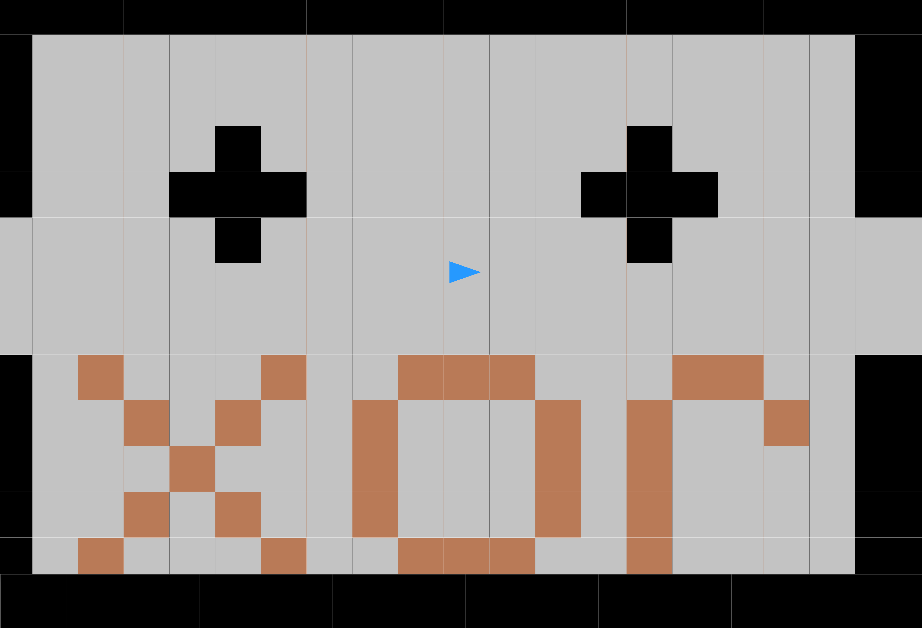
\includegraphics[width=.7\linewidth]{figures/project.png}
\end{center}
}

\frameT{Any Questions?} {
 
  \begin{center}
    Questions?
  \end{center}
  
  \begin{center}
    Comments?
  \end{center}

  \bigskip
  
  \begin{center}
  Author information:
  \end{center}  

	\begin{center}
	Steven Gray (https://github.com/steagray)  
	James Nail (https://github.com/LoganBrown559)
	Logan Brown (https://github.com/jamesnail)  
	\end{center}

  \begin{center}
		Repo:
    https://github.com/steagray/FA22-Senior-Design
  \end{center}
}

%\frameF{fragile test} {
%}

%% \frameF{Prolog Family Tree} {
%% \begin{verbatim}
%% hello
%% \end{verbatim}



%% }

%Empty Page
%\frameT{Frame 1}{
%}  


\end{document}
